\documentclass[11pt,a4paper]{article}
\usepackage[utf8]{inputenc}
\usepackage[T1]{fontenc}
\usepackage[spanish,es-nodecimaldot]{babel}
\usepackage{lmodern}
\usepackage{amsmath}
\usepackage{graphicx}
\usepackage{booktabs}
\usepackage{float}
\usepackage[margin=2.3cm]{geometry}
\usepackage{xcolor}
\usepackage{caption}
\usepackage[colorlinks=true,linkcolor=blue!50!black,urlcolor=blue!50!black]{hyperref}
\captionsetup{font=small,labelfont=bf}
\graphicspath{{../figuras/}}
\newcommand{\aviso}[1]{\par\smallskip\noindent\fcolorbox{orange!70!black}{orange!8}{\parbox{\dimexpr\linewidth-2\fboxsep-2\fboxrule}{\small #1}}\par\smallskip}
\usepackage{url}
\makeatletter\g@addto@macro{\UrlBreaks}{\do\-\do\_\do\.}\makeatother
\urlstyle{tt}\DeclareRobustCommand{\archivo}[1]{\path{#1}}

\title{Análisis del espectro de la fuente de neutrones $^{241}$Am-Be\\
\large usada como entrada de MEIGA (carpeta \texttt{Simulacion-fuente-241AmBe})}
\author{Jaime Betancourt}
\date{19 de octubre de 2026}

\begin{document}
\maketitle

\begin{abstract}
Se revisó la cadena completa con la que se construyó la fuente de neutrones $^{241}$Am-Be para MEIGA:
el espectro digitalizado, la conversión a número de neutrones por energía, el archivo final de
1\,637\,458 neutrones en formato CORSIKA/ARTI y las curvas de referencia usadas en las figuras.
La conversión energía$\to$momento y el formato son correctos y la energía media del archivo
(4.06~MeV) está cerca del valor ISO~8529-1 (4.16~MeV). Pero el método tiene cuatro defectos: (i) cada
\emph{punto digitalizado} se trató como una energía discreta con peso $\propto S(E)$, de modo que el
número de neutrones por intervalo sigue la \emph{densidad de puntos} del digitalizador (sesgos de
$-46$\,\% a $+35$\,\% en bins de 0.25~MeV); (ii) entran 28 puntos espurios (6.2\,\% de los
neutrones); (iii) el espectro es un peine de 437 líneas; y (iv) el archivo está ordenado según la
digitalización, así que una corrida que use solo las primeras líneas recibe neutrones de baja energía.
Además, la curva rotulada ``IAEA (referencia)'' no es un espectro IAEA/ISO, y la segunda digitalización
tiene el eje $y$ invertido (la inversión de columna del notebook no la corrige). Con los puntos válidos
se construyó un espectro limpio $S(E)$ con $\langle E\rangle=4.15$~MeV (ISO: 4.16~MeV) y estructura
en 3.0, 4.9, 6.3, 7.5 y 9.5~MeV, y se generó una fuente corregida (energías continuas, orden
aleatorio, mismo formato), validada con $\chi^2/\mathrm{ndf}=218/214$.
Además se digitalizó el espectro de referencia ISO~8529 desde la figura de la norma publicada por el IAEA
(47 grupos, $\langle E\rangle=4.21$~MeV), que resultó ser el mismo espectro de la digitalización previa.
Con él se generó la irradiación del tanque por una fuente de 1~Ci durante 5~minutos a 10~cm de la pared:
202\,363\,865 neutrones que entran al tanque (de 665\,980\,683 emitidos), en formato \texttt{eFromFile} de MEIGA.
\end{abstract}

\tableofcontents

%==========================================================================
\section{Archivos revisados y cadena de construcción}

El análisis lee los archivos originales sin modificarlos. Todo lo nuevo está en
\archivo{Simulacion-fuente-241AmBe/Analisis-fuente-AmBe/} (\archivo{scripts/}, \archivo{figuras/},
\archivo{resultados/}, \archivo{informe/}).

\begin{table}[H]
\centering\small
\caption{Archivos de la carpeta y su papel. Las líneas se cuentan con \texttt{wc -l}.}
\label{tab:archivos}
\begin{tabular}{p{6.0cm}p{9.0cm}}
\toprule
Archivo & Contenido / papel \\
\midrule
\archivo{espectro-neutrones-Am-Be-241.txt} (\archivo{-clean}) & Digitalización principal: 667 pares $(E, y)$ con coma decimal (la versión \archivo{-clean} usa punto). \textbf{Es la base de la fuente.}\\
\archivo{espectro_procesado_frecuencia(_redondeado).txt} & $y\times 2.5\times10^{6}$, redondeado a entero y con $|\cdot|$: número de neutrones por punto (suma 1\,637\,458).\\
\archivo{Espectro-energia-neutrones-AmBe-241.txt} & Cada energía repetida $n_i$ veces (1\,637\,458 líneas).\\
\archivo{Espectro-completo-neutrones-fuente-AmBe241.txt} & \textbf{Fuente MEIGA}: \texttt{13 0 0 pz 0 0 0 0 0 0 0 0}, $p_z$ en GeV/c.\\
\archivo{Datos-originales-espectro-AmBe-241.txt} = \archivo{Default-Dataset-2.csv} & Segunda digitalización (472 puntos, ordenada); \archivo{Datos-mejorados-...} es la misma con punto decimal.\\
\archivo{Funcion-espectro-AmBe-241(-final).txt} & La segunda digitalización con la columna $y$ invertida en orden (\S\ref{sec:segunda}).\\
\archivo{AmBe_IAEA.txt}, \archivo{AmBe_ISO8529_spectrum.txt}, \archivo{AmBe_neutron_spectrum.txt} & Curvas de ``referencia'' (\S\ref{sec:referencias}).\\
\archivo{neutron_0MeV.txt}, \archivo{neutron_500MeV.txt}, \archivo{neutrones_4710_0.10327MeV.txt}, \archivo{neutrones_generados.txt} & Pruebas de formato monoenergéticas.\\
\archivo{simulacion-241-AmBe.ipynb} & Construye la cadena anterior (celdas 1--13); el resto son análisis de otros temas (acero, procesos gamma).\\
\archivo{Espectro-energia-AmBe-241.ipynb}, \archivo{Distancias-capturas-neutrones.ipynb} & Histogramas del archivo de energías y comparación con \archivo{AmBe_IAEA.txt}.\\
\bottomrule
\end{tabular}
\end{table}

La cadena del notebook \archivo{simulacion-241-AmBe.ipynb} es:
\[
(E_i, y_i)\ \xrightarrow{\ \times 2.5\cdot10^{6},\ \mathrm{round},\ |\cdot|\ }\ n_i\ \xrightarrow{\ \text{repetir } n_i \text{ veces}\ }\ \{E\}\ \xrightarrow{\ p=\sqrt{(T+m_n)^2-m_n^2}\ }\ \texttt{13 0 0 }p_z\ldots
\]
con $m_n=939.565$~MeV/c$^2$. Se verificó que el archivo final tiene 1\,637\,458 líneas, todas con
identificador CORSIKA 13 (neutrón), $p_x=p_y=0$ y posiciones nulas. La energía cinética reconstruida desde
$p_z$ coincide con el archivo de energías con un error máximo de 0.07~keV (efecto de imprimir $p_z$ con
6 cifras significativas). \textbf{El formato y la cinemática son correctos.}

%==========================================================================
\section{Diagnóstico de la digitalización principal}

\begin{figure}[H]
\centering
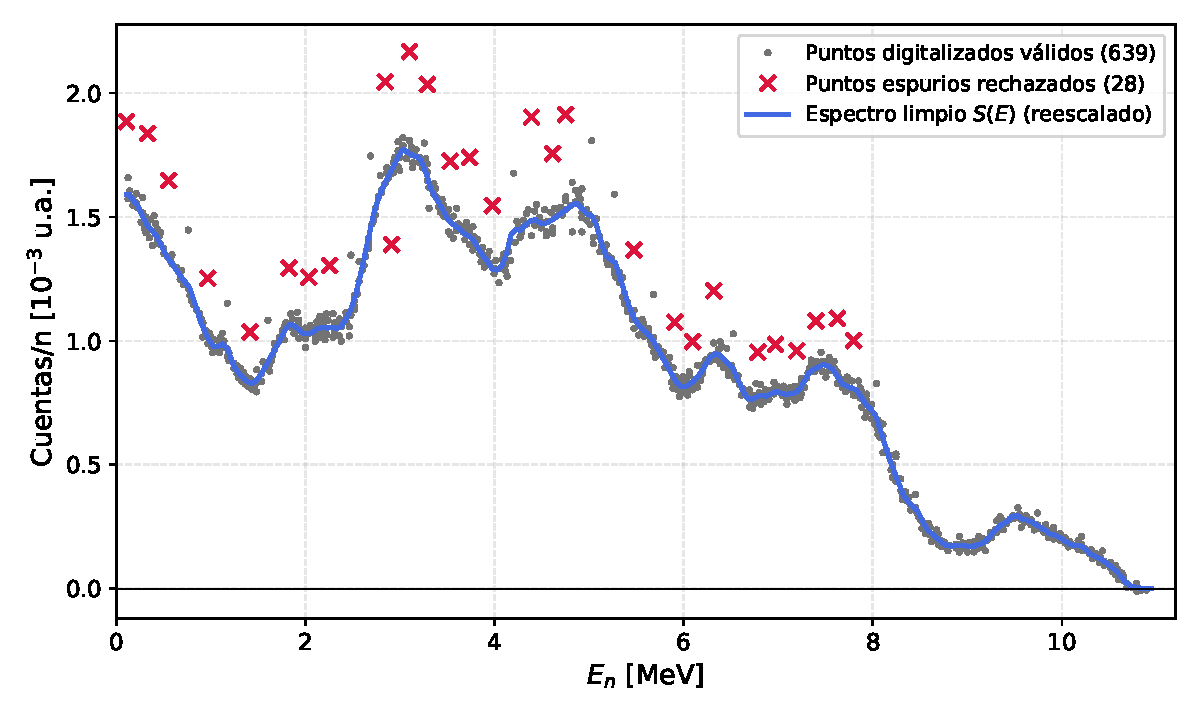
\includegraphics[width=0.92\linewidth]{fig01_digitalizacion_espurios.pdf}
\caption{Digitalización principal (667 puntos). Las cruces son los 28 puntos rechazados (se apartan de la mediana local en $\pm0.15$~MeV más de $\max(3.5\,\mathrm{MAD},\,10^{-4})$). La línea azul es el espectro limpio $S(E)$ de la \S\ref{sec:limpio}, reescalado a las unidades de la digitalización.}
\label{fig:dig}
\end{figure}

La digitalización es automática (tipo WebPlotDigitizer) y tiene las imperfecciones habituales:
\begin{itemize}
\item \textbf{No está ordenada en energía}: 193 de los 666 pasos retroceden en $E$, y solo hay 437 energías distintas (hay energías repetidas con distintos $y$ y 4 pares exactamente repetidos). La Fig.~\ref{fig:orden} muestra que el digitalizador recorrió la curva en varias pasadas: tramos que vuelven a 0.3--1.6~MeV (líneas 179--186) y un grupo final de 18 puntos (líneas 649--666) entre 0.1 y 5~MeV.
\item \textbf{28 puntos espurios} (Fig.~\ref{fig:dig}), muy por encima de la curva: probablemente marcadores sueltos o el símbolo de la leyenda. Juntos representan el 6.2\,\% de los neutrones de la fuente (101\,100 neutrones).
\item \textbf{3 valores negativos} cerca de 10.8~MeV, convertidos en positivos con \texttt{np.abs} (55 neutrones; efecto despreciable, pero conceptualmente deberían ser cero).
\item La digitalización empieza en 0.103~MeV: la fuente no tiene neutrones por debajo de 0.1~MeV.
\end{itemize}

\begin{figure}[H]
\centering
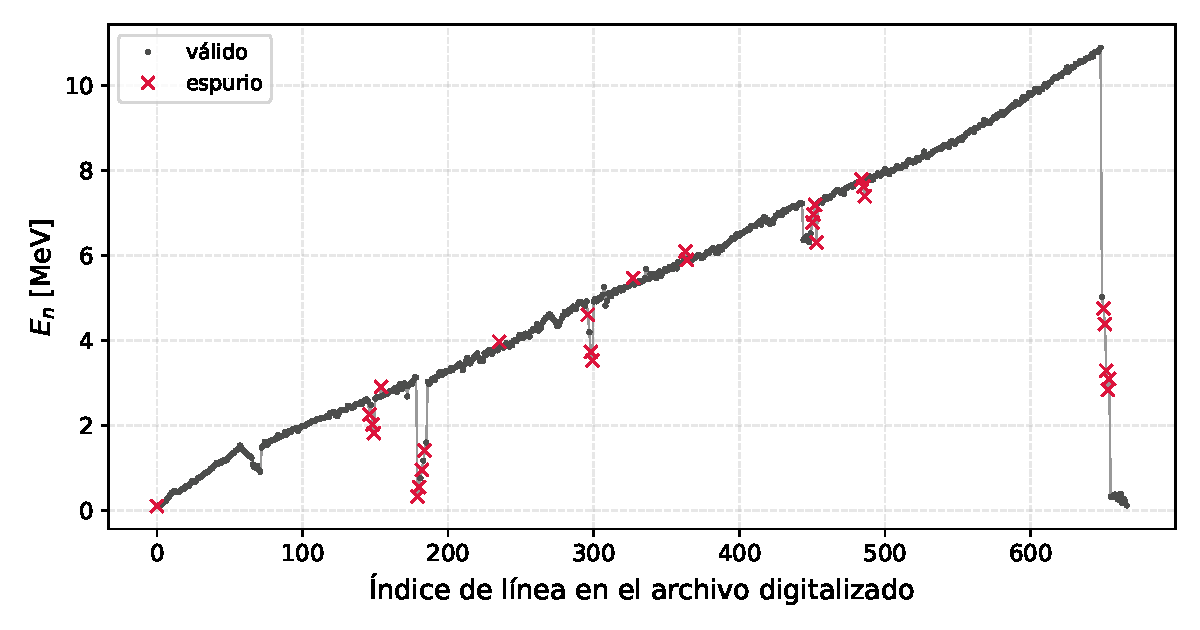
\includegraphics[width=0.85\linewidth]{fig02_orden_digitalizacion.pdf}
\caption{Energía de cada punto en el orden del archivo digitalizado. El orden del archivo se hereda tal cual en la fuente MEIGA (\S\ref{sec:orden}).}
\label{fig:orden}
\end{figure}

%==========================================================================
\section{Espectro limpio y comparación con ISO 8529-1}
\label{sec:limpio}

Con los 639 puntos válidos (negativos llevados a cero) se promedió en bins de 0.05~MeV, se interpoló
en los bins vacíos, se aplicó un suavizado binomial de 3 bins (solo para quitar el ruido de
digitalización) y se normalizó a área 1 entre 0.10 y 10.95~MeV. El resultado, $S(E)$ en MeV$^{-1}$ en una
malla de 5~keV, está en \archivo{resultados/espectro_AmBe_limpio.txt}.

\begin{table}[H]
\centering\small
\caption{Propiedades del espectro limpio y de las dos fuentes. $\langle E\rangle_\text{ISO}=4.16$~MeV es la energía media de fluencia del espectro de referencia $^{241}$Am-Be de ISO~8529-1.}
\label{tab:prop}
\begin{tabular}{lccc}
\toprule
 & $S(E)$ limpio & Fuente original MEIGA & Fuente corregida \\
\midrule
$\langle E\rangle$ [MeV] & 4.152 & 4.064 & 4.151 \\
Mediana [MeV] & 3.99 & 3.84 & 3.99 \\
Energías distintas & continuo & 437 & 1\,311\,568 \\
\midrule
Fracción 0.1--1 MeV [\%] & 12.08 & 12.14 & 12.09 \\
Fracción 1--2 MeV [\%]  & 9.60 & 9.58 & 9.61 \\
Fracción 2--4 MeV [\%]  & 28.51 & 30.61 & 28.49 \\
Fracción 4--6 MeV [\%]  & 26.23 & 25.30 & 26.25 \\
Fracción 6--8 MeV [\%]  & 16.89 & 16.81 & 16.89 \\
Fracción 8--11 MeV [\%] & 6.69 & 5.55 & 6.68 \\
\bottomrule
\end{tabular}
\end{table}

El espectro limpio tiene máximos locales en \textbf{3.03, 4.88, 6.33, 7.47 y 9.53~MeV}, una
componente que crece hacia bajas energías por debajo de 1~MeV y el corte en $\approx10.8$~MeV. Esta es la
forma del espectro $^{241}$Am-Be (reacción $^9$Be$(\alpha,n)^{12}$C con $^{12}$C en el estado fundamental y
en los estados excitados de 4.44 y 7.65~MeV). Su energía media, 4.15~MeV, coincide con la de ISO~8529-1
(4.16~MeV) a menos del 0.3\,\%.

\aviso{\textbf{Procedencia.} No hay en la carpeta un registro de qué figura (artículo, ISO~8529-1,
otra simulación) se digitalizó para \archivo{espectro-neutrones-Am-Be-241.txt}. La etiqueta del eje
original (``Cuentas/n'') sugiere un histograma por neutrón. Para la tesis hay que citar esa fuente.
La coincidencia de $\langle E\rangle$ con ISO 8529-1 indica que es un espectro Am-Be realista.}

%==========================================================================
\section{La fuente cargada en MEIGA}

\subsection{Sesgo por la densidad de puntos digitalizados}

El paso clave del notebook asigna a \emph{cada punto} $i$ un número de neutrones $n_i\propto y_i$, todos
con la energía $E_i$. Eso solo reproduce el espectro si los puntos están uniformemente espaciados en
$E$. El número correcto de neutrones en un intervalo es $\int S(E)\,dE \approx S(E_i)\,\Delta E_i$. Con
espaciado irregular, el número de neutrones en un intervalo es $\sum_{i\in\text{bin}} y_i$, proporcional al
\emph{número de puntos} que el digitalizador puso en ese intervalo.

\begin{figure}[H]
\centering
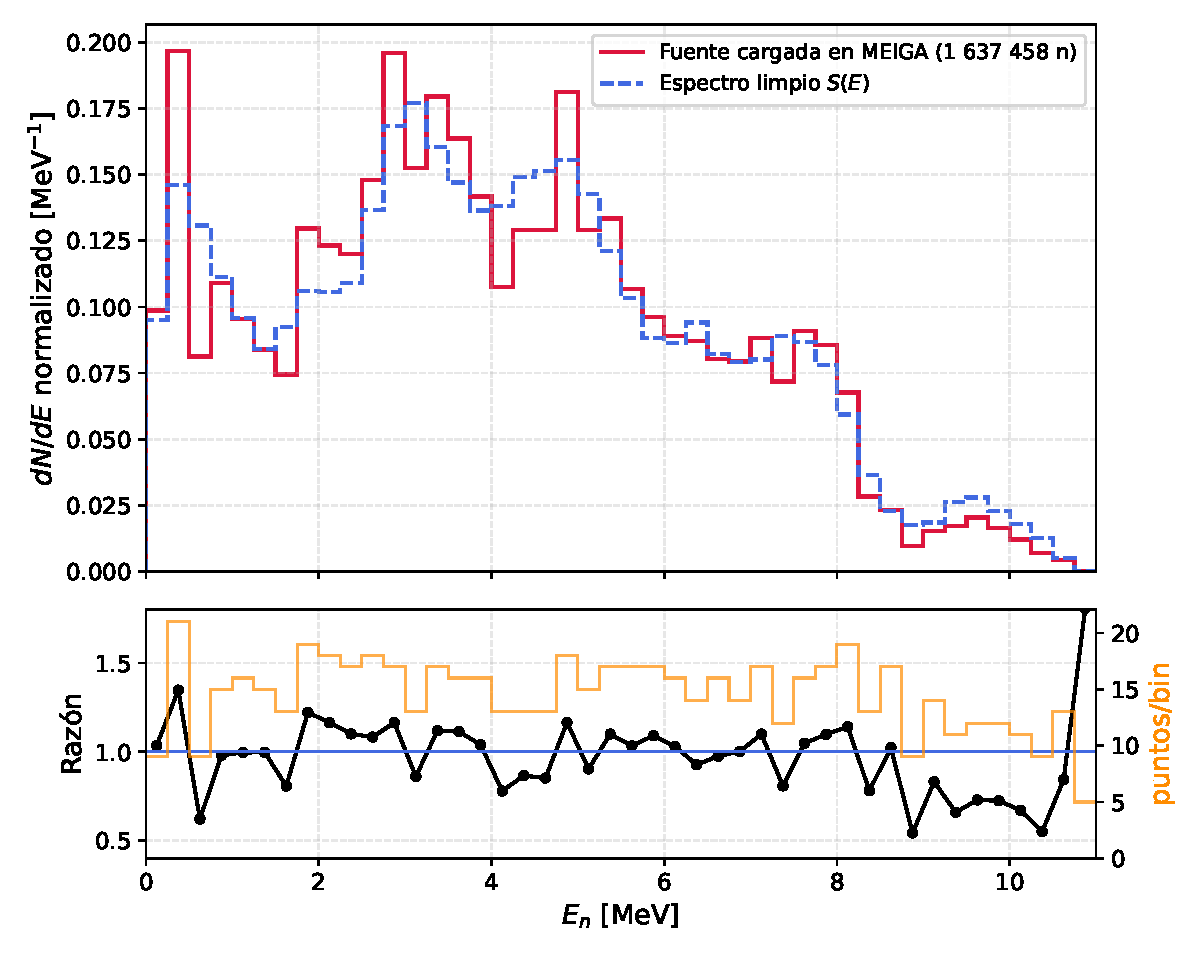
\includegraphics[width=0.85\linewidth]{fig03_fuente_vs_limpio.pdf}
\caption{Arriba: espectro de energía de la fuente MEIGA original (reconstruido desde $p_z$) frente al espectro limpio, en bins de 0.25~MeV. Abajo: razón fuente/limpio (negro) y número de puntos digitalizados válidos por bin (naranja). La correlación entre ambas curvas es 0.97.}
\label{fig:sesgo}
\end{figure}

La Fig.~\ref{fig:sesgo} muestra el efecto: la razón fuente/limpio va de 0.54 a 1.35 y sigue casi
exactamente (correlación 0.97) al número de puntos por bin. Por ejemplo, el bin 0.25--0.5~MeV tiene 21
puntos (más los espurios) y queda un 35\,\% alto, mientras que la región 8.5--10.5~MeV, digitalizada con
menos puntos, queda entre un 17 y un 46\,\% baja. En conjunto (Tabla~\ref{tab:prop}), la fuente original tiene
2.1~puntos porcentuales de más en 2--4~MeV y un 17\,\% menos de neutrones por encima de 8~MeV, y su energía
media es 0.09~MeV (2\,\%) menor.

\subsection{Espectro discreto: origen de los picos en ``Geant4 (suavizado)''}

\begin{figure}[H]
\centering
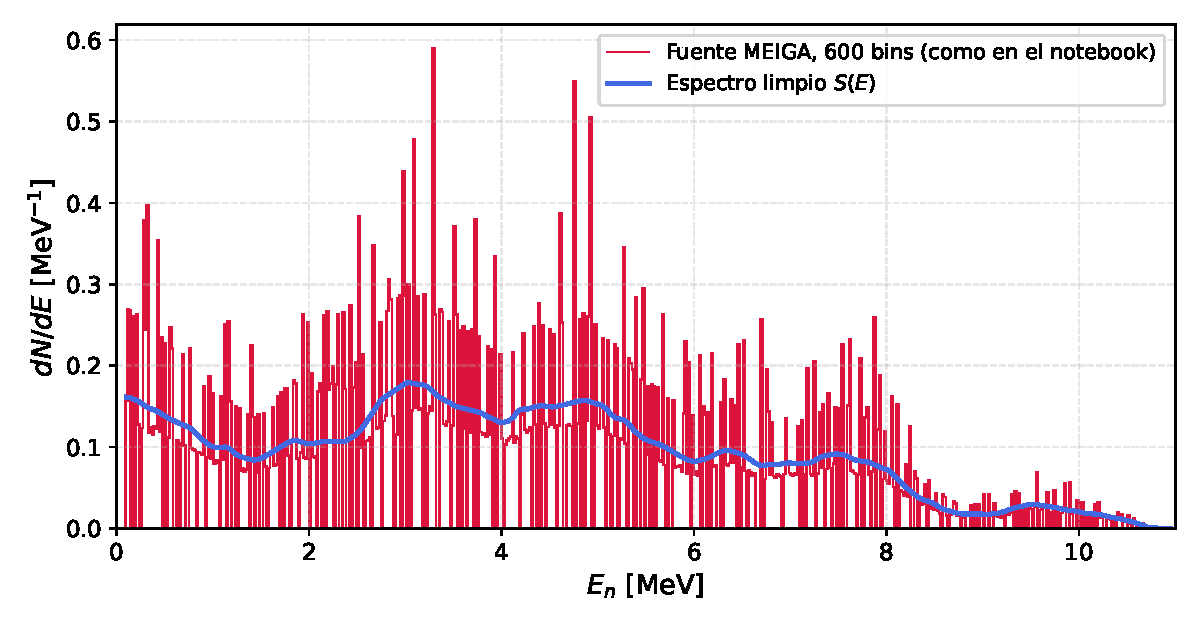
\includegraphics[width=0.88\linewidth]{fig04_fuente_discreta.pdf}
\caption{La fuente original en 600 bins (como en \archivo{Espectro-energia-AmBe-241.ipynb}): un peine de 437 energías discretas. Muchos bins quedan vacíos y otros reciben 2--3 líneas.}
\label{fig:discreta}
\end{figure}

Como todas las energías son las 437 abscisas digitalizadas, un histograma fino de la fuente es un peine
(Fig.~\ref{fig:discreta}). El suavizado gaussiano de 1.5--1.8 bins de las figuras
\archivo{Espectro-AmBe-241-suavizado} y \archivo{Espectro-AmBe-Geant4-vs-IAEA} no basta para borrarlo. Las
oscilaciones de la curva azul de esas figuras (picos de 0.24 en 0.3 y 3.3~MeV) son en gran parte este
artefacto, sumado al sesgo de la sección anterior; no son estructura física.

\aviso{\textbf{Etiqueta incorrecta.} En esas figuras la curva se rotula ``Geant4'', pero lo que se
histograma es \archivo{Espectro-energia-neutrones-AmBe-241.txt}, es decir, el \emph{archivo de entrada}
construido en Python, no una salida de Geant4/MEIGA. Para hablar del espectro ``visto por Geant4'' habría
que histogramar la energía del primario registrada por MEIGA. Del mismo modo,
\archivo{Espectros-energia-AmBe-241.png} conserva rótulos heredados de otro notebook (``Rayleigh 1 meV'',
``Agua pura'').}

\subsection{Orden del archivo}
\label{sec:orden}

\begin{figure}[H]
\centering
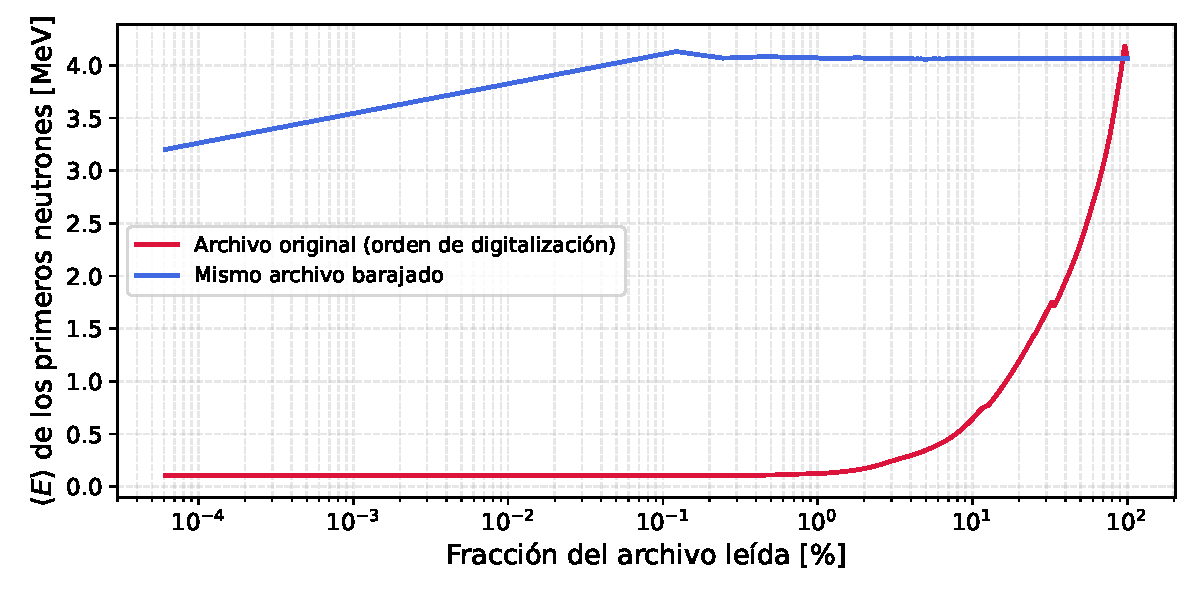
\includegraphics[width=0.85\linewidth]{fig07_sesgo_orden.pdf}
\caption{Energía media de los primeros $k$ neutrones del archivo en función de la fracción leída. En el archivo original las energías salen en el orden de la digitalización; barajado (azul), cualquier subconjunto tiene ya el espectro completo.}
\label{fig:ordenfig}
\end{figure}

El archivo escribe los $n_i$ neutrones de cada punto en bloque y en el orden de la digitalización. Si
una corrida de MEIGA lee solo las primeras $N$ líneas (prueba corta, corrida interrumpida, o un archivo
recortado con \texttt{head}, como en otras corridas de la tesis), el espectro queda fuertemente sesgado
(Fig.~\ref{fig:ordenfig}):

\begin{center}\small
\begin{tabular}{lcc}
\toprule
Primeras líneas & $\langle E\rangle$ [MeV] & $E_\text{max}$ [MeV] \\
\midrule
1\,\% (16\,374 n) & 0.12 & 0.14 \\
10\,\% & 0.64 & 1.34 \\
25\,\% & 1.44 & 2.62 \\
50\,\% & 2.32 & 4.17 \\
100\,\% & 4.06 & 10.90 \\
\bottomrule
\end{tabular}
\end{center}

\aviso{\textbf{A verificar.} Si alguna corrida de MEIGA ya usó este archivo con menos de los
1\,637\,458 neutrones, sus resultados corresponden a un espectro de baja energía y no a Am-Be.}

\subsection{Dirección y posición}

Todos los neutrones tienen $p_x=p_y=0$ y $p_z>0$ en el archivo: un haz pincel. En el código de MEIGA
(\archivo{IO/ParticleFiller.cc}) el momento leído se guarda como $(p_x,\,p_y,\,-p_z)$, así que en Geant4
estos neutrones viajan en $-z$, \textbf{hacia abajo}. Con \texttt{eCircle}/\texttt{eVertical} la posición
la fija \archivo{DetectorList.xml} (las columnas $x,y,z$ del archivo, en cm, solo se usan con
\texttt{eFromFile}). Una fuente Am-Be real emite de forma isótropa. El haz vertical puede ser una
elección deliberada (incidencia normal, como en las corridas monoenergéticas), pero conviene declararlo.
El generador corregido admite \texttt{--direccion iso}; sus opciones \texttt{+z}/\texttt{-z} se refieren
al signo escrito en el archivo, no a la dirección en Geant4.

%==========================================================================
\section{Segunda digitalización: eje $y$ invertido}
\label{sec:segunda}

\begin{figure}[H]
\centering
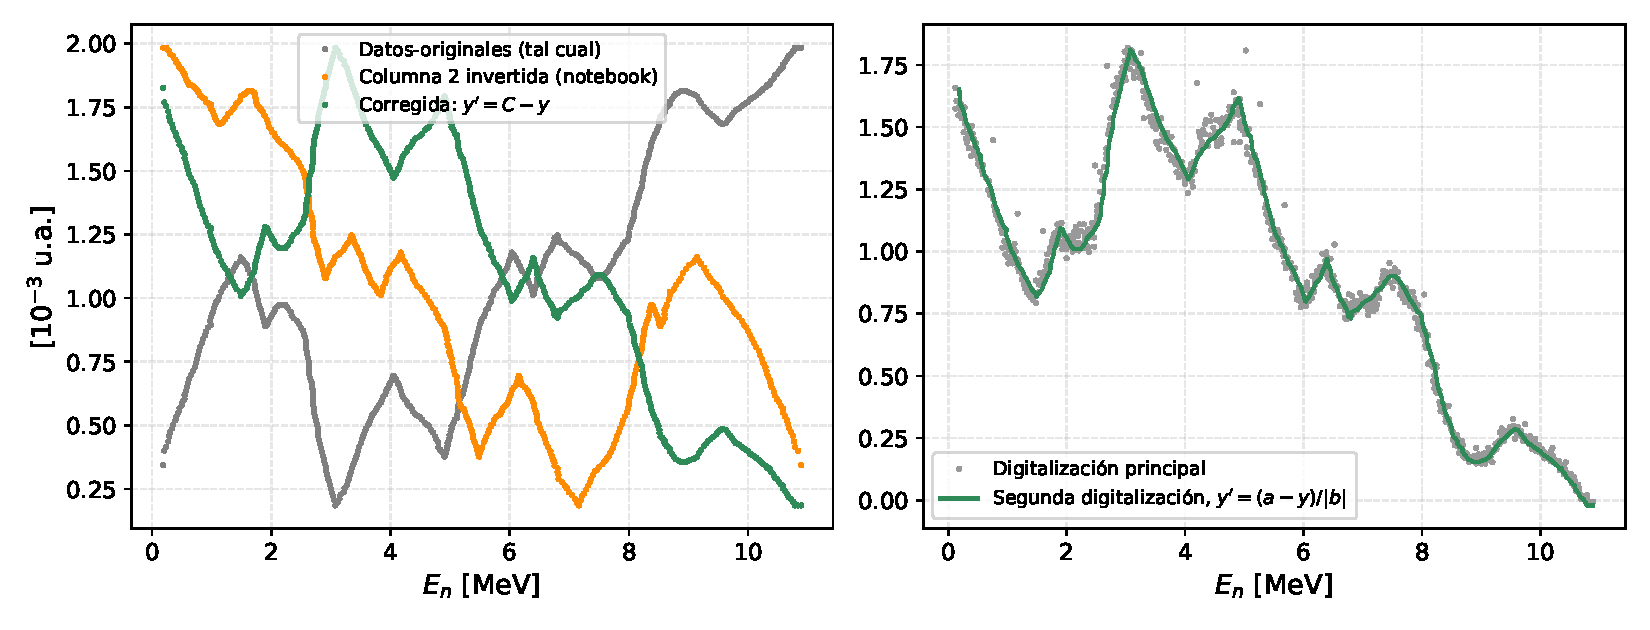
\includegraphics[width=\linewidth]{fig05_segunda_digitalizacion.pdf}
\caption{Izquierda: \archivo{Datos-originales} tal cual (gris), con la columna $y$ invertida en orden como en el notebook (naranja), y como $C-y$ (verde). Derecha: la inversión lineal ajustada $y'=(a-y)/|b|$ coincide con la digitalización principal.}
\label{fig:segunda}
\end{figure}

La segunda toma (\archivo{Datos-originales-espectro-AmBe-241.txt}, 472 puntos) crece con la energía y tiene
mínimos donde el espectro real tiene máximos (3.0 y 4.9~MeV). Su correlación con $S(E)$ es
$-0.997$: es el mismo espectro con el \textbf{eje $y$ calibrado al revés} en el digitalizador. El ajuste
lineal $y=a+b\,S(E)$ da $a=1.96\times10^{-3}$, $b=-9.69\times10^{-3}$, y $y'=(a-y)/|b|$ reproduce la
digitalización principal (Fig.~\ref{fig:segunda}, derecha).

La corrección del notebook (\texttt{col2[::-1]}, archivo \archivo{Funcion-espectro-AmBe-241-final.txt})
invierte el \emph{orden} de la columna, lo que equivale a reflejar el espectro en energía
($E\to E_\text{min}+E_\text{max}-E$). La curva resultante decrece con $E$, pero tiene los picos en
posiciones equivocadas (correlación con $S(E)$: solo 0.32). La figura
\archivo{Funcion-espectro-energia-Am-Be-241.png} muestra esta segunda toma \emph{sin} corregir. Ninguna
de las dos variantes entra en la fuente MEIGA, pero no deben usarse ni citarse.

%==========================================================================
\section{Las curvas de ``referencia''}
\label{sec:referencias}

\begin{figure}[H]
\centering
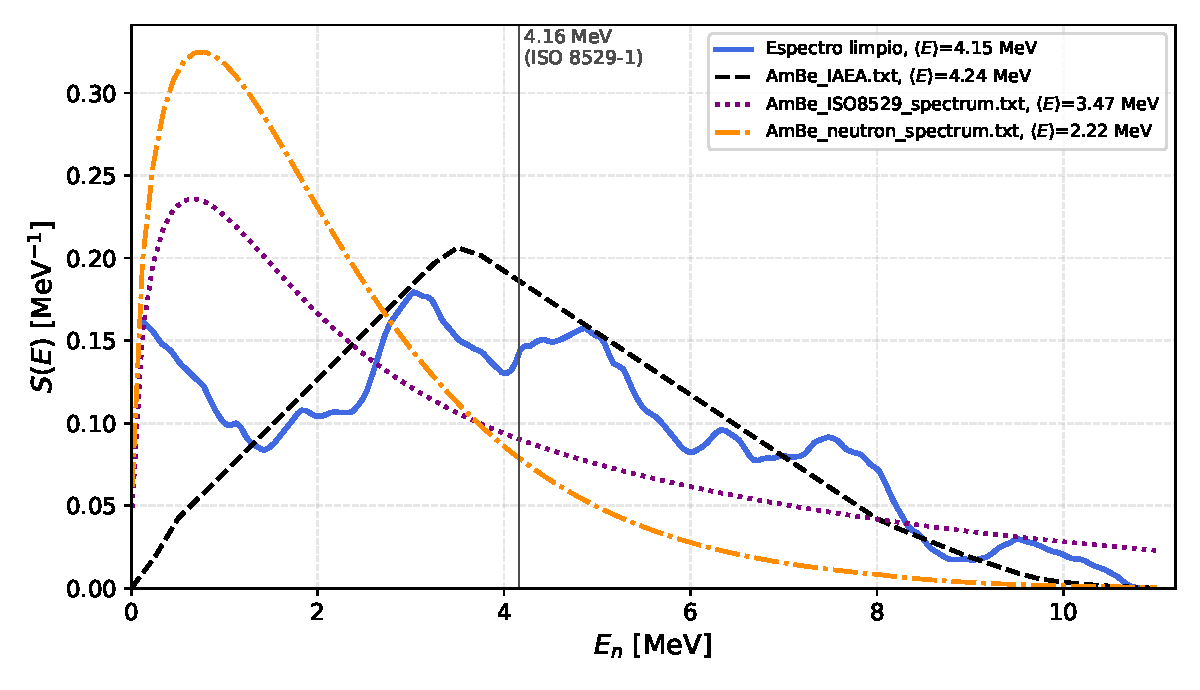
\includegraphics[width=0.88\linewidth]{fig06_referencias.pdf}
\caption{Espectro limpio frente a los tres archivos de referencia de la carpeta (todos normalizados a área 1). La línea vertical marca la energía media ISO 8529-1.}
\label{fig:refs}
\end{figure}

\begin{itemize}
\item \archivo{AmBe_IAEA.txt} (usada como ``IAEA (referencia)'' en \archivo{Espectro-AmBe-Geant4-vs-IAEA}): 45 puntos cada 0.25~MeV con valores redondos (0.020, 0.045, \ldots) que forman un triángulo con un único máximo en 3.5~MeV. \textbf{No es un espectro tabulado de IAEA ni de ISO}: no tiene ninguna de las estructuras del Am-Be. Coincide con la media ISO solo de forma aproximada (4.24~MeV), por construcción.
\item \archivo{AmBe_ISO8529_spectrum.txt} y \archivo{AmBe_neutron_spectrum.txt}: 100 puntos en una malla lineal de 0.111~MeV con forma analítica suave (tipo Maxwell/Watt) y un máximo cerca de 0.7~MeV. Sus energías medias (3.47 y 2.22~MeV) están lejos de 4.16~MeV. \textbf{Tampoco son el espectro ISO 8529-1}, pese al nombre.
\end{itemize}

\aviso{Para comparar con una referencia real hay que usar la tabla del Anexo A de ISO~8529-1 (edición vigente,
que incluye fuentes Am-Be pequeñas y grandes) o el compendio IAEA TRS-403. Se sabe que los espectros Am-Be
medidos difieren del ISO entre 3 y 6~MeV y cerca de 8~MeV, según la cápsula y la mezcla. Mientras tanto, la
única comparación cuantitativa defendible es $\langle E\rangle$ = 4.15 frente a 4.16~MeV.}

%==========================================================================
\section{Fuente corregida y validación}

\archivo{scripts/generar_fuente.py} muestrea $S(E)$ por inversión exacta de la función acumulada
(interpolación lineal por tramos). Cada neutrón tiene una energía continua, los neutrones salen en orden
aleatorio y el formato es el mismo del original:
\begin{verbatim}
python3 scripts/generar_fuente.py      # 1637458 n, +z, semilla 2026
python3 scripts/generar_fuente.py -n 150000 --direccion iso --semilla 7
\end{verbatim}
El archivo por defecto \archivo{resultados/Fuente-AmBe241-corregida-1637458n.txt} (59~MB) reemplaza
directamente a \archivo{Espectro-completo-neutrones-fuente-AmBe241.txt}. Junto a él se escribe la lista
de energías (\archivo{-energias.txt}).

\begin{figure}[H]
\centering
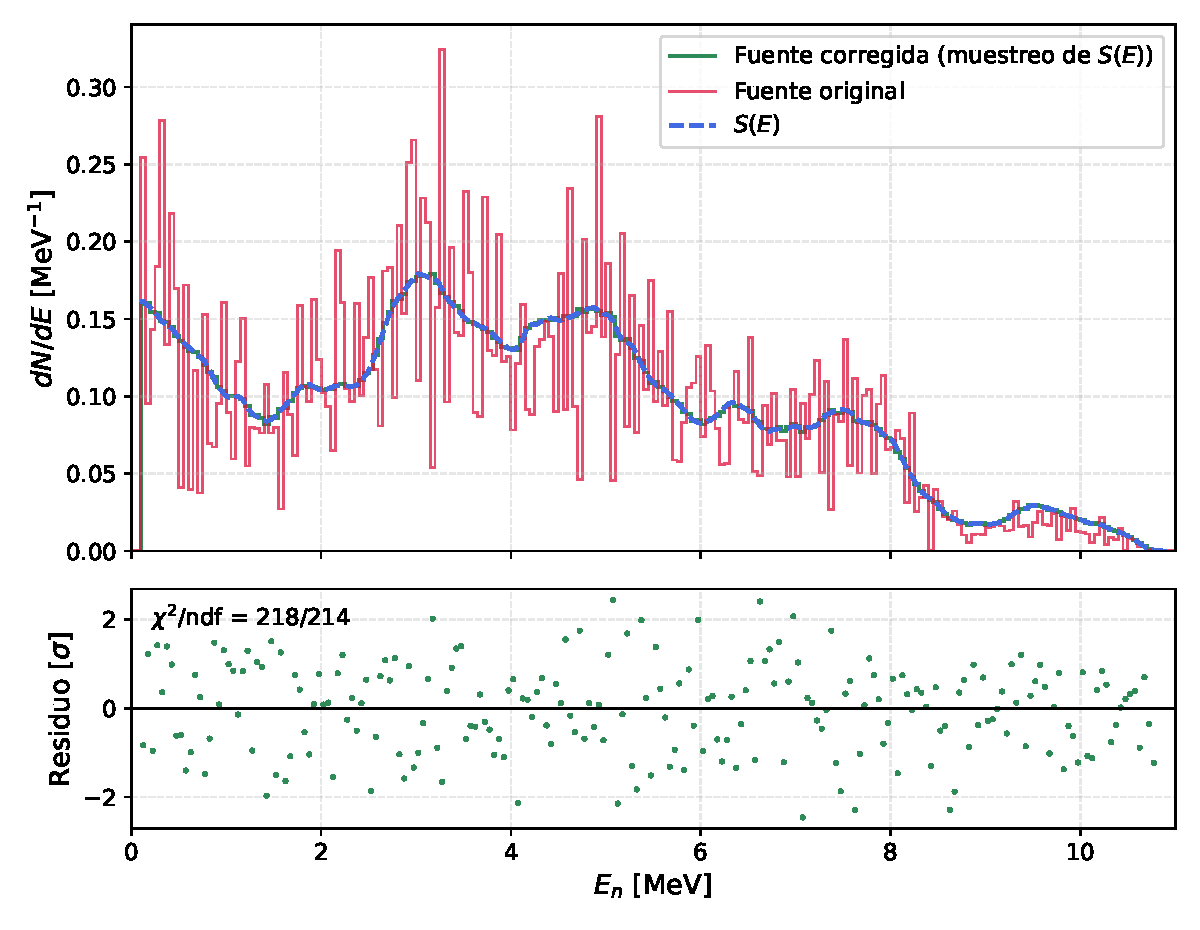
\includegraphics[width=0.85\linewidth]{fig08_validacion_fuente_corregida.pdf}
\caption{Validación de la fuente corregida (energía reconstruida desde el momento, bins de 0.05~MeV) frente a $S(E)$, con la fuente original como comparación. Abajo: residuos en desviaciones estándar.}
\label{fig:valid}
\end{figure}

\archivo{scripts/validar_fuente.py} relee el archivo, reconstruye $T$ desde $|\vec p|$ y compara con
$S(E)$: $\chi^2/\mathrm{ndf}=218/214$, $\langle E\rangle=4.151$~MeV (esperado 4.152) y residuos sin
estructura (Fig.~\ref{fig:valid}). El primer 1\,\% del archivo ya tiene $\langle E\rangle = 4.17$~MeV,
así que se puede usar cualquier subconjunto inicial.

%==========================================================================
\section{Espectro de referencia ISO 8529 digitalizado}
\label{sec:iso}

Para tener una referencia real se buscó el espectro $^{241}$Am-Be de ISO~8529. Las tablas del Anexo de la
norma no son de acceso libre. La figura de la norma ($B_E\cdot E$ frente a $E_n$, histograma en escala
logarítmica) aparece en la lámina~26 de la presentación del IAEA \emph{Establishing neutron calibrations at
SSDL using ISO 8529 radionuclide sources}\footnote{\url{https://ssdl.iaea.org/Content/IAEA\%20lecture\%20on\%20Establishing\%20neutron\%20calibrations\%20at\%20SSDL.pdf}}.
La lámina indica una fuente de $3.0\times10^{6}$~n/s con cápsula X3. La imagen original (1191$\times$790~px)
se guardó en \archivo{referencia_ISO8529/}.

\paragraph{Digitalización.} \archivo{scripts/digitalizar_iso8529.py} reconstruye el histograma
directamente desde los píxeles:
\begin{itemize}
\item Eje $y$: ajuste lineal a las marcas 0, 0.2, 0.4, 0.6 y 0.8 (residuos $<1$~px).
\item Eje $x$: las décadas del dibujo tienen anchos distintos (297, 273 y 284~px), así que $\log_{10}E$ se
interpola linealmente entre \emph{todas} las marcas detectadas (29 marcas entre 0.01 y 20~MeV).
\item Trazo: en cada columna se mide el intervalo vertical ocupado por la línea, de 4~px de grueso. Por
encima de 5~MeV muchos escalones son más angostos que el trazo vertical (5~px). Para resolverlos se usa
que el intervalo de la columna $c$ es $[\min S,\max S]$ de la escalera en $[c-2,\,c+2]$. El nivel en $x$
es la intersección de los intervalos de las columnas vecinas, y los picos y valles angostos se toman de
los extremos locales de esos intervalos.
\end{itemize}
El resultado son \textbf{47 grupos entre 0.100 y 10.84~MeV}
(\archivo{resultados/ISO8529_AmBe_digitalizado.txt}). La superposición sobre la imagen
(Fig.~\ref{fig:isodig}) reproduce todos los escalones; solo se pierde el último escalón de
$\approx0.02$ entre 10.84 y 10.9~MeV (contribución $<0.05$\,\%).

\begin{figure}[H]
\centering
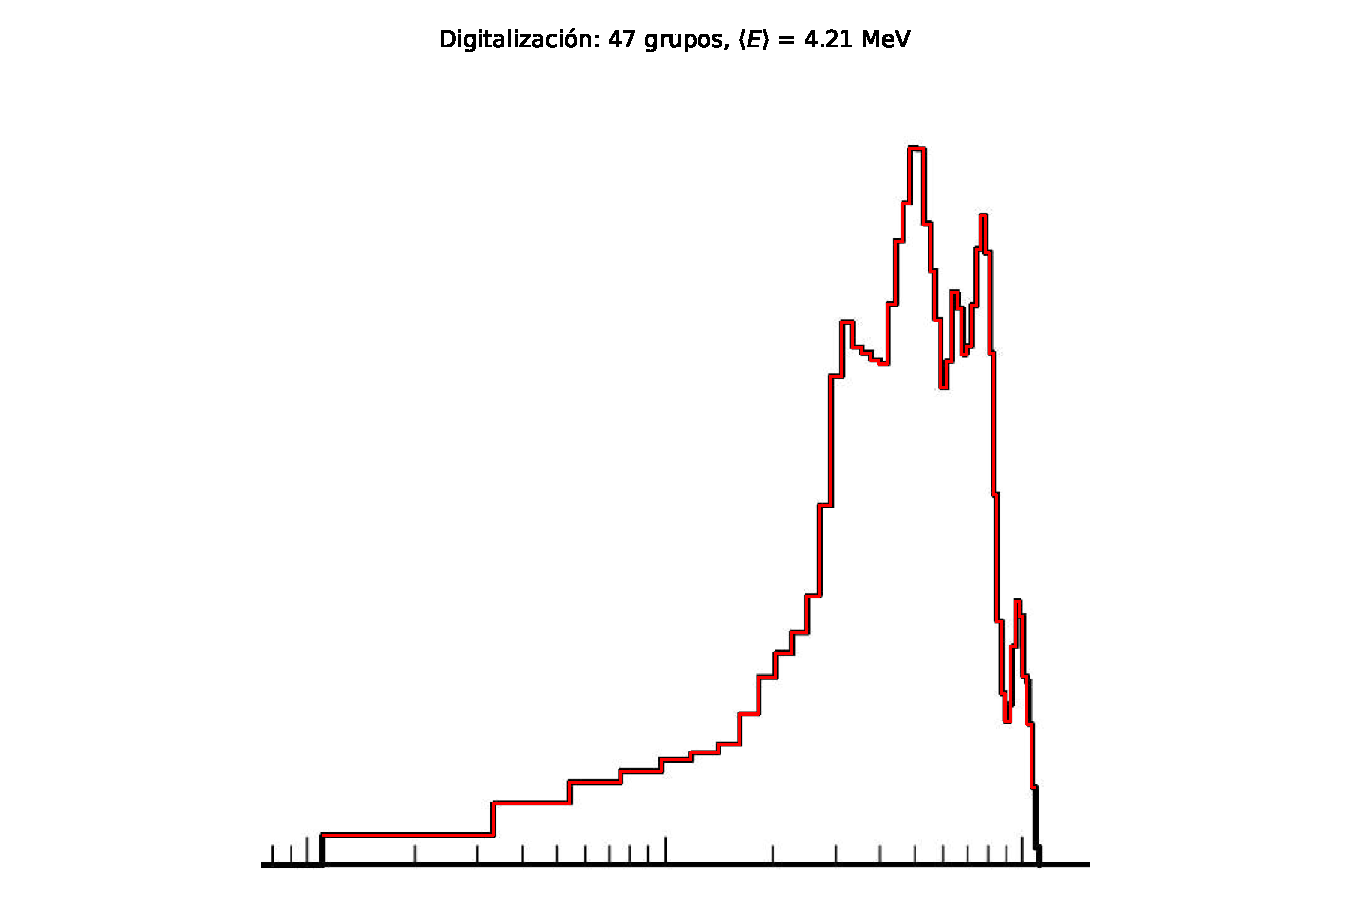
\includegraphics[width=0.78\linewidth]{fig09_digitalizacion_ISO8529.pdf}
\caption{Digitalización (rojo) superpuesta a la figura ISO 8529 de la lámina IAEA (negro).}
\label{fig:isodig}
\end{figure}

\paragraph{Validación.} Tomando $B_E\cdot E$ constante dentro de cada grupo, la energía media de fluencia
del espectro digitalizado es $\langle E\rangle=4.21$~MeV. La norma da 4.16~MeV (ISO 8529-1:2001) y,
en la edición 2021, 4.17~MeV para la fuente ``pequeña'' y 4.05~MeV para la ``grande''. La diferencia del
1\,\% es compatible con la resolución del dibujo y con la forma supuesta dentro de cada grupo.

\begin{figure}[H]
\centering
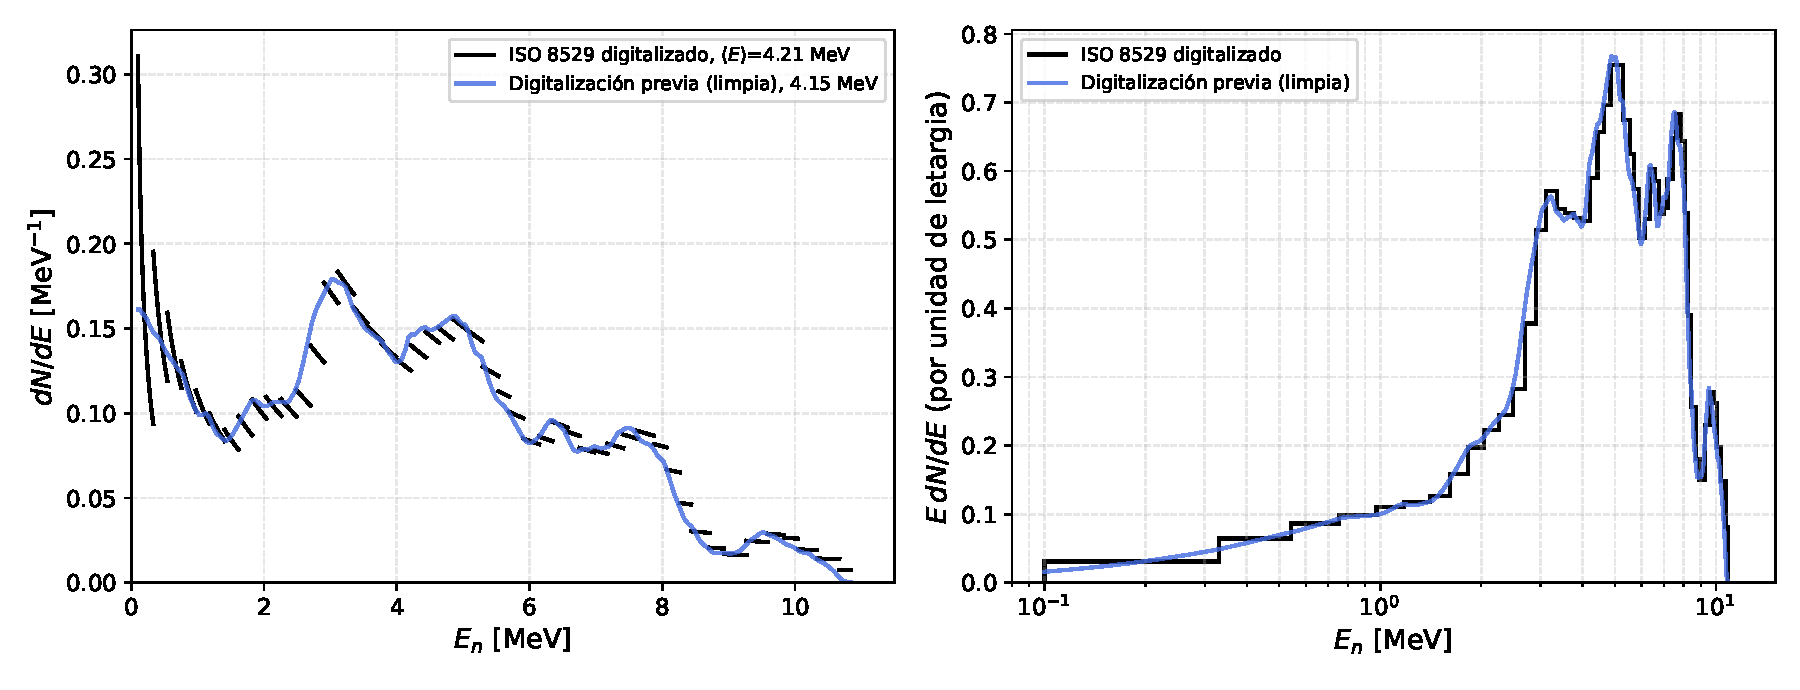
\includegraphics[width=\linewidth]{fig10_iso8529_vs_previa.pdf}
\caption{Espectro ISO 8529 digitalizado (negro) frente al espectro limpio de la digitalización previa de la carpeta (azul). Izquierda: $dN/dE$ (dentro de cada grupo ISO, $dN/dE\propto1/E$). Derecha: por unidad de letargia.}
\label{fig:isoprev}
\end{figure}

\begin{table}[H]
\centering\small
\caption{Fracción de neutrones por banda de energía.}
\label{tab:bandas_iso}
\begin{tabular}{lcccccc}
\toprule
Banda [MeV] & 0.1--1 & 1--2 & 2--4 & 4--6 & 6--8 & 8--11 \\
\midrule
ISO 8529 digitalizado [\%] & 12.57 & 9.40 & 27.40 & 26.09 & 16.87 & 7.66 \\
Digitalización previa (limpia) [\%] & 12.08 & 9.60 & 28.51 & 26.23 & 16.89 & 6.69 \\
\bottomrule
\end{tabular}
\end{table}

La Fig.~\ref{fig:isoprev} y la Tabla~\ref{tab:bandas_iso} muestran que \textbf{la digitalización previa de
la carpeta es este mismo espectro ISO}, convertido a $dN/dE$: mismos picos y mismas fracciones por banda,
con diferencias de alrededor de 1 punto porcentual. Esto resuelve la duda de procedencia de la
\S\ref{sec:limpio}. Para la tesis conviene citar ISO~8529-1 y usar la versión digitalizada aquí, que
conserva los grupos originales.

%==========================================================================
\section{Irradiación del tanque: 1 Ci durante 5 minutos a 10 cm}
\label{sec:irradiacion}

\paragraph{Intensidad.} ISO 8529-1:2021 (Tabla~1) da para $^{241}$Am-Be una emisión específica indicativa
de $6\times10^{-5}$~n\,s$^{-1}$\,Bq$^{-1}$. Para 1~Ci ($3.7\times10^{10}$~Bq) esto da
$Q=2.22\times10^{6}$~n/s. En 300~s se emitieron $N=$~665\,980\,683 neutrones en $4\pi$, número sorteado de
una distribución de Poisson de media $Q\,t$. Como la norma advierte, el valor real depende de cada fuente;
si se conoce la emisión calibrada de la fuente, basta con cambiar \texttt{--rendimiento} o
\texttt{--actividad-Ci}.

\paragraph{Geometría.} Se usa el tanque de la réplica de Sidelnik (\texttt{eSaltyWCD}): agua de
$R=48$~cm y $H=133$~cm, Tyvek de 0.12~mm y acero de 0.5~mm, de modo que $R_\text{ext}=48.062$~cm. El
fondo exterior está en $z=0$ y la tapa exterior en $z=133.124$~cm. La fuente es puntual e isótropa, a
10~cm de la pared exterior y a media altura del agua: $\vec r_s=(-58.062,\,0,\,66.562)$~cm. Solo se
escriben los neutrones cuya dirección corta el tanque. Desde un punto fuera del cilindro y a una altura
dentro de él, un rayo solo puede entrar por la pared lateral, así que basta con la intersección
rayo-cilindro. La fracción geométrica es $f=0.30386\pm0.00002$, comprobada de forma independiente por marcha de
rayos ($0.3040\pm0.0010$). Así, \textbf{202\,363\,865 neutrones} llegan al tanque, es decir,
$6.75\times10^{5}$~n/s.

\paragraph{Archivos.} En \archivo{resultados/Irradiacion-AmBe-1Ci-300s-d10cm/} hay 203 partes de
$10^{6}$ neutrones (15~GB en total) más \archivo{resumen.json}. Cada línea es
\verb|13 px py pz x y z 0 0 0 0 0| ($p$ en GeV/c, posición en cm). Como \archivo{ParticleFiller.cc}
de MEIGA guarda $(p_x,p_y,-p_z)$, el generador escribe $-p_z$ para que la dirección en Geant4 sea la
correcta. MEIGA debe usar \texttt{injectionMode eFromFile} para leer la posición de cada línea; hay un
ejemplo en \archivo{configuracion/DetectorList-AmBe-d10cm.xml}. Las partes son muestras aleatorias
independientes del total, así que cualquier subconjunto es representativo.

\begin{figure}[H]
\centering
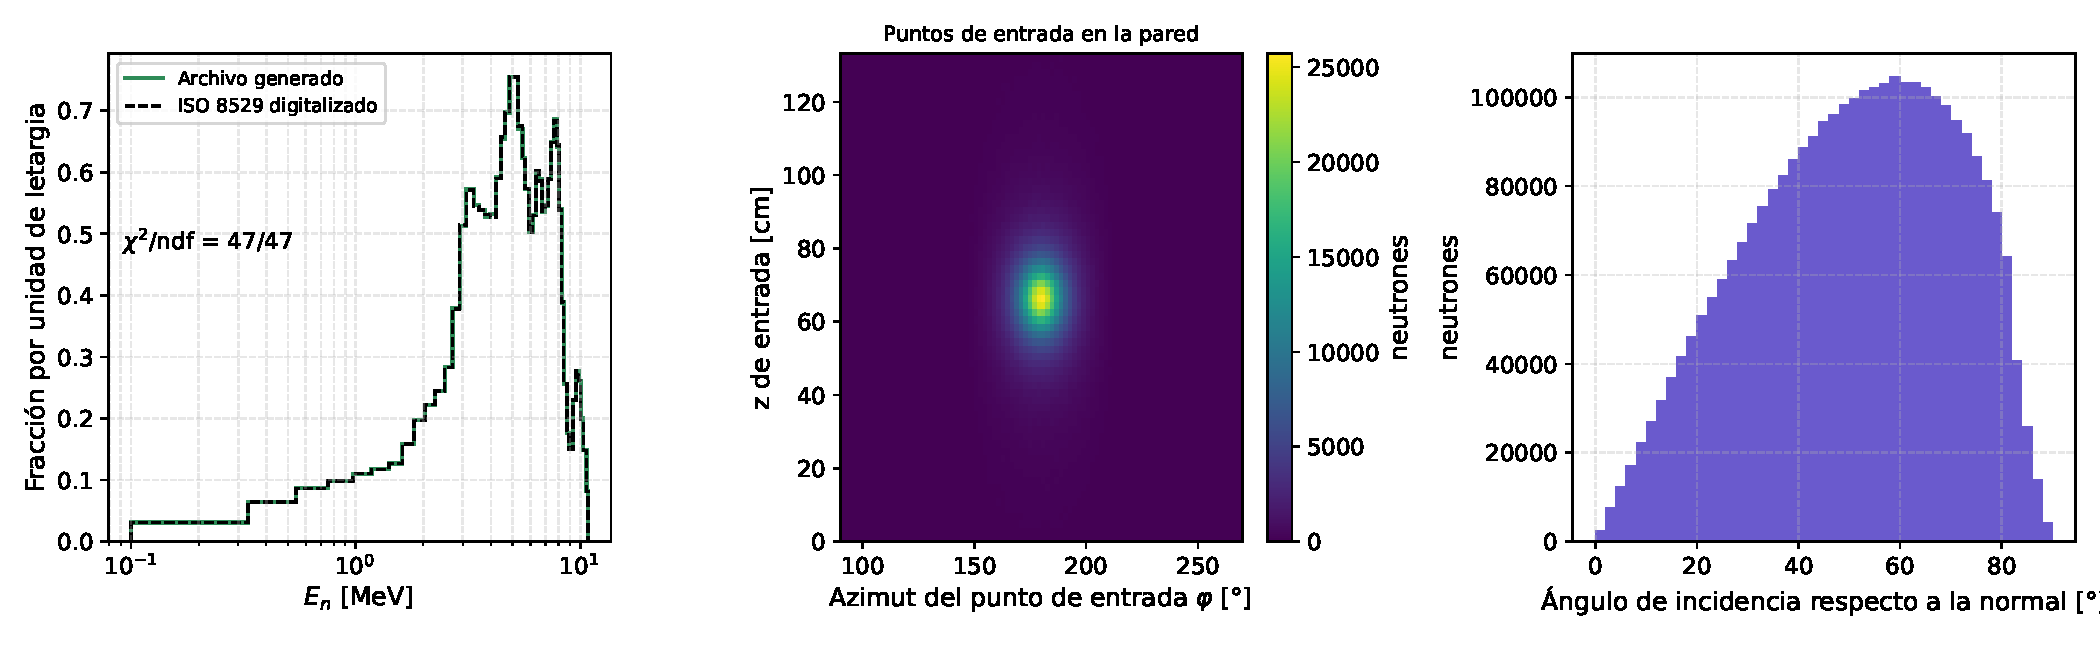
\includegraphics[width=\linewidth]{fig11_validacion_irradiacion.pdf}
\caption{Validación de $3\times10^{6}$ neutrones de 3 partes elegidas al azar. Izquierda: espectro reconstruido desde el momento frente al ISO digitalizado. Centro: puntos de entrada en la pared lateral ($\varphi=180^\circ$ mira a la fuente). Derecha: ángulo de incidencia respecto a la normal de la pared.}
\label{fig:irr}
\end{figure}

\paragraph{Validación.} \archivo{scripts/validar_irradiacion.py} relee tres partes al azar, deshace la
inversión de $p_z$ y comprueba lo siguiente: todas las posiciones son la de la fuente; el
100\,\% de los rayos entra al tanque; $\langle E\rangle=$~4.210~MeV (esperado 4.211); y el
espectro por grupo da $\chi^2/\mathrm{ndf}=$~47/47. Los puntos de entrada se concentran frente a la
fuente y el ángulo medio de incidencia es 50$^\circ$ (Fig.~\ref{fig:irr}).

\aviso{\textbf{Costo y uso en MEIGA.} 202\,363\,865 neutrones primarios es mucho más de lo que se puede
simular completo: las corridas de 150\,000 neutrones de 500~MeV tardaron ~20~h. Lo práctico es simular
una o varias partes ($10^6$ neutrones cada una), medir la tasa de lo que interese (capturas, carga,
eficiencia) por neutrón incidente y escalar a los 5~min multiplicando por $N_\text{tanque}/N_\text{simulados}$.
Hay que medir antes la velocidad de MEIGA con una parte de prueba.}

\aviso{\textbf{Limitaciones.} (1) MEIGA simula cada neutrón como un evento independiente y el archivo no
lleva tiempos de emisión. Con $6.75\times10^{5}$~n/s entrando y $\tau_\text{captura}\approx200~\mu$s, en el tanque
real hay del orden de $10^{2}$ neutrones moderándose a la vez (apilamiento). Si interesa la señal en el
tiempo, hay que asignar tiempos con un proceso de Poisson en el análisis. (2) No se simulan los neutrones
que no apuntan al tanque (el 70\,\%), así que se desprecia el retorno por dispersión en suelo, aire y
paredes del recinto, que en un laboratorio real puede aportar una fracción apreciable de neutrones
térmicos. (3) La fuente es puntual y sin cápsula, con la anisotropía y la atenuación de la cápsula
despreciadas. (4) No se incluyen los gammas de 4.44~MeV ($\approx0.6$ por neutrón)
Am-Be, ni los de 59.5~keV del $^{241}$Am.}

%==========================================================================
\section{Montaje blindado: haz, halo y fondo}
\label{sec:blindado}

\paragraph{Montaje.} La fuente está dentro de una caja de polietileno/parafina, al fondo de un canal
cilíndrico de 3~cm de diámetro y 30~cm de largo que apunta al tanque. Entre la caja y el tanque hay
10~cm de plomo (bloques de $10\times40\times120$~cm), y todo está sobre una mesa, a media altura del
tanque. La fuente queda entonces a 40~cm de la pared exterior, en $(-88.062,\,0,\,66.562)$~cm.

\paragraph{Haz geométrico.} El canal deja un cono de semiángulo $\arctan(1.5/30)=2.86^\circ$
($5.7^\circ$ en total). Eso es el $0.062$\,\% de la emisión, 1\,385~n/s, y produce una mancha de 4~cm
de diámetro ($\approx12.6$~cm$^2$, el 0.10\,\% de la silueta del tanque). Con el canal de 5~cm el cono
sería de $9.5^\circ$ (0.173\,\%, 35~cm$^2$). Una estimación por atenuación exponencial
(\archivo{scripts/blindaje_fuga.py}, caja supuesta como cubo de 60~cm) da entre $4\times10^4$ y
$7.5\times10^5$ neutrones rápidos al tanque en 5~min. Según esa estimación, el haz es solo
${\sim}17$\,\% de ellos y el resto es fuga por el polietileno. La incertidumbre (factor ${\sim}17$)
muestra que el blindaje requeriría una simulación de transporte.

\paragraph{Modelo adoptado.} En lugar de simular el transporte, el autor fijó tres componentes,
expresadas como fracción de los neutrones que entran al tanque
(\archivo{scripts/generar_irradiacion_compuesta.py}):
\begin{center}\small
\begin{tabular}{p{2.2cm}cp{3.4cm}p{6.3cm}}
\toprule
Componente & Fracción & Energía & Origen y dirección \\
\midrule
Haz directo & 35\,\% & ISO 8529 (0.1--10.8 MeV) & desde la fuente, cono de $2.86^\circ$ \\
Halo difuso & 45\,\% & 0.5 eV--100 keV, $1/E$ & cara del plomo ($120\times40$ cm), 0--$90^\circ$, ley del coseno \\
Fondo hemisférico & 20\,\% & $10^{-4}$--0.5 eV, flujo maxwelliano ($kT$ = 25.3 meV) & plano frente al tanque ($96\times133$ cm), isótropo en el hemisferio \\
\bottomrule
\end{tabular}
\end{center}
El maxwelliano reparte el fondo en 26\,\% entre $10^{-4}$ y 0.025~eV y 74\,\% entre 0.025 y 0.5~eV.
La normalización se ancla en el haz: $Q\cdot\Omega/4\pi\cdot T_\text{Pb}\cdot t$, con
$T_\text{Pb}=e^{-0.116\cdot10}=0.313$ (remoción), da $1.30\times10^{5}$ neutrones de haz en 5~min. El total
es entonces $1.30\times10^5/0.35$.

\paragraph{Resultado.} El archivo
\archivo{resultados/Irradiacion-AmBe-blindada-1Ci-300s/373272N-Irradiacion-AmBe-blindada-1Ci-300s.txt}
(29~MB) tiene \textbf{373\,272 neutrones}: 130\,711 de haz, 167\,963 de halo y 74\,598 de fondo. Eso
equivale a 1\,244~n/s, el 0.056\,\% de lo emitido. Las líneas están barajadas. La columna~8 marca la
componente (1, 2 o 3); MEIGA la lee pero no la usa. Además, \archivo{-componentes.txt} da la componente
y la energía de cada línea (línea $k$ = \texttt{run\_id} $k$). Se usa con \texttt{eFromFile}, igual que
antes. La validación (\archivo{scripts/validar_irradiacion_compuesta.py}) confirma que todos los
neutrones entran al tanque y que las fracciones son 35.0/45.0/20.0\,\%. Al calcular el momento se evitó
la cancelación numérica de $\sqrt{(E+m)^2-m^2}$ a energías térmicas: la energía reconstruida coincide a
$10^{-6}$.

\begin{figure}[H]
\centering
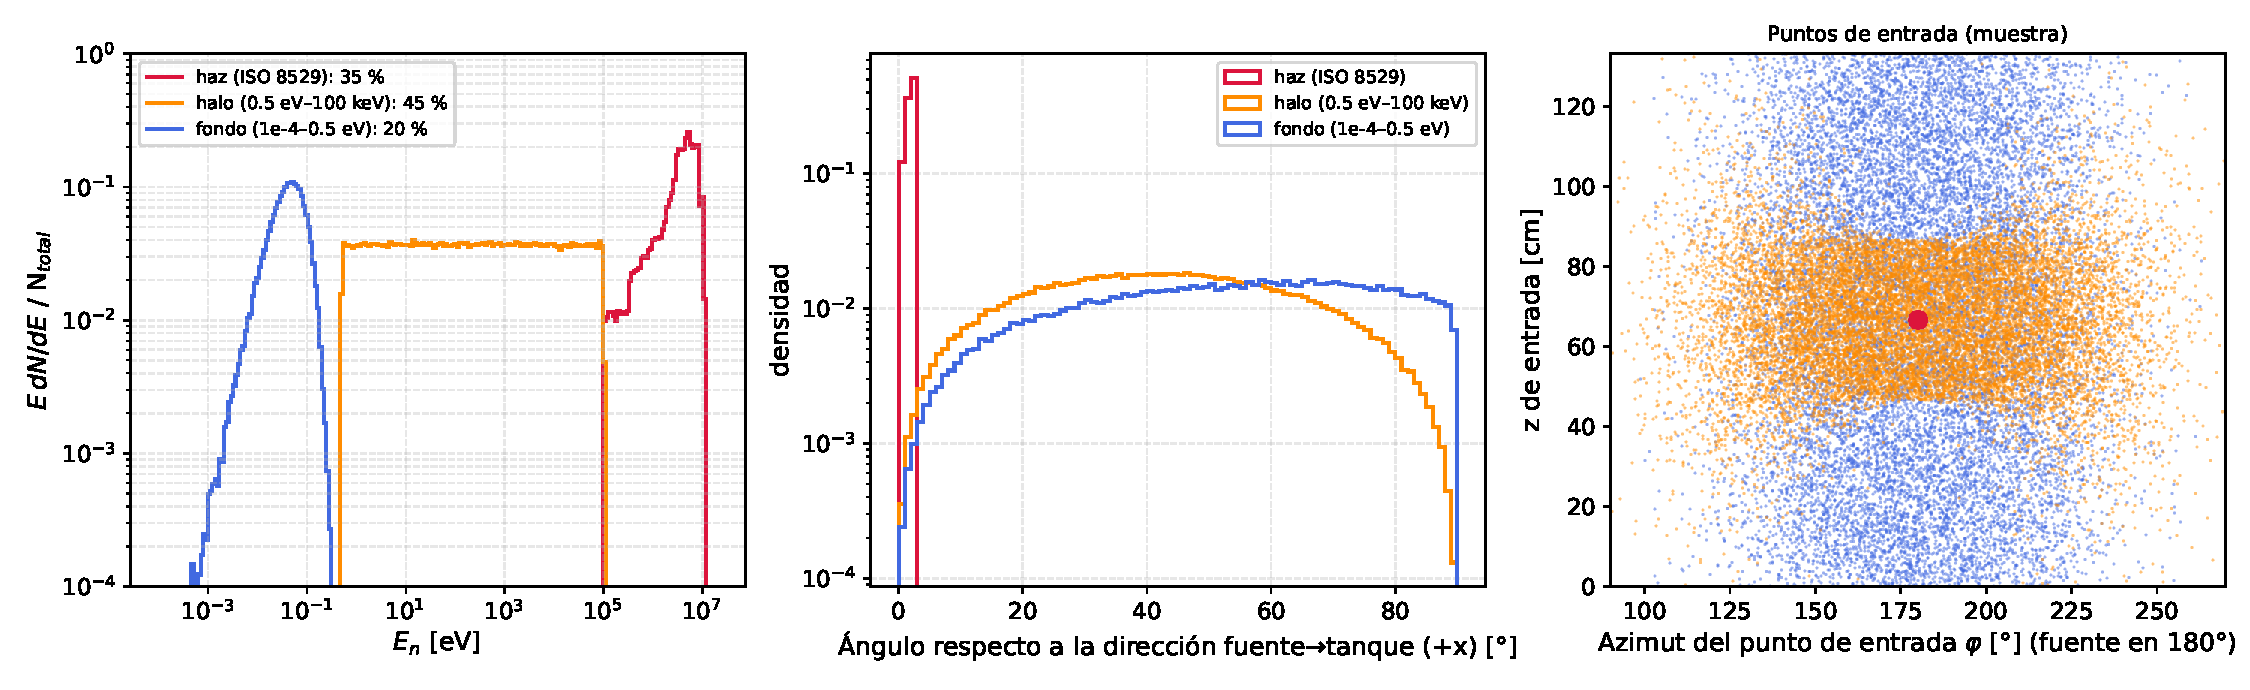
\includegraphics[width=\linewidth]{fig12_irradiacion_compuesta.pdf}
\caption{Archivo compuesto: espectro por componente (por unidad de letargia), ángulo respecto a la dirección fuente$\to$tanque y puntos de entrada en la pared (muestra).}
\label{fig:compuesta}
\end{figure}

\aviso{\textbf{Decisiones de modelado (revisables con opciones del script).} Hay tres elecciones
de modelado. (1) El haz se ancla con $T_\text{Pb}=0.313$; con la transmisión sin choque (0.082) todo
se reduce $\times0.26$ (\texttt{--T-plomo}). (2) El halo sale uniforme de la cara del plomo y el fondo
de un plano de $96\times133$~cm; un halo concentrado alrededor del haz cambiaría los puntos de entrada,
no el número. (3) Las fracciones 35/45/20 se pueden cambiar con \texttt{--fracciones}. El haz no
incluye la degradación de energía al cruzar el plomo.}

%==========================================================================
\section{Conclusiones y recomendaciones}

\begin{enumerate}
\item La conversión energía$\to$momento (GeV/c) y el formato CORSIKA/ARTI de la fuente original son correctos.
\item El espectro digitalizado, una vez limpio, es un espectro $^{241}$Am-Be realista: $\langle E\rangle = 4.15$~MeV frente a 4.16~MeV de ISO 8529-1, con estructura en 3.0, 4.9, 6.3, 7.5 y 9.5~MeV.
\item La fuente original distorsiona ese espectro porque reparte los neutrones según la densidad de puntos digitalizados ($-46$\,\% a $+35$\,\% por bin de 0.25~MeV; $-17$\,\% por encima de 8~MeV; $\langle E\rangle$ 2\,\% baja), incluye 28 puntos espurios (6.2\,\% de los neutrones) y es un peine de 437 energías. Los picos de las figuras ``Geant4 (suavizado)'' son artefactos de esto, y la etiqueta ``Geant4'' es incorrecta.
\item El archivo original está ordenado: cualquier corrida que use solo parte de él simula un espectro de baja energía. \textbf{Hay que verificar si alguna corrida ya lo usó así.}
\item \archivo{AmBe_IAEA.txt} y los dos archivos ``ISO8529'' no son espectros de referencia; no deben presentarse como IAEA/ISO en la tesis.
\item La segunda digitalización tiene el eje $y$ invertido; la corrección del notebook (invertir el orden de la columna) es incorrecta.
\item Se recomienda usar \archivo{Fuente-AmBe241-corregida-1637458n.txt} (o generar el $N$ y la dirección necesarios), declarar en la tesis la procedencia de la figura digitalizada y la geometría de emisión, y, si se quiere una comparación con referencia, digitalizar o tabular el Anexo A de ISO 8529-1.
\item El espectro ISO 8529 se digitalizó desde la figura de la norma en una lámina del IAEA (47 grupos, $\langle E\rangle=4.21$~MeV frente a 4.16--4.17~MeV). La digitalización previa de la carpeta resultó ser ese mismo espectro.
\item Para irradiar el tanque con 1~Ci durante 5~min a 10~cm se generaron 202\,363\,865 neutrones (30.3\,\% de los 665\,980\,683 emitidos), listos para MEIGA con \texttt{eFromFile}. Conviene simular una muestra de las partes y escalar.
\item Para el montaje blindado (canal de 3~cm, 10~cm de plomo) y el modelo haz/halo/fondo (35/45/20\,\%) llegan al tanque 373\,272 neutrones en 5~min, el 0.056\,\% de lo emitido. Caben en una sola corrida de MEIGA.
\end{enumerate}

\end{document}
